\section{Experiment}
The experiment aims at using reinforcement learning algorithms for solid-state lidar with steerable rays and a limited number of rays. At first, it was necessary to create an environment where the agent can learn and evaluate \cite{rozsypalek2018}. The lidar-gym environment is written in python 3 based on OpenAI gym interface \cite{openai2016}. It uses point clouds from Kitti dataset drives\cite{geiger2013}. One episode of learning in environment corresponds to one drive in Kitti dataset. Large point clouds from drives are processed into 3D voxel maps by C++ package \cite{petricek2017}, which also provides ray tracing engine for the environment. Every voxel map is a 3D array containing real numbers which correspond to the occupancy confidence $c$ of each voxel.
\begin{align}
\begin{split}
c &> 0 \quad \text{occupied voxel} \\
c &= 0 \quad \text{unknown occupancy} \\
c &< 0 \quad \text{empty voxel.}
\end{split}
\end{align}
The environment also offers visualization of actions using Mayavi \cite{mayavi2011} and ASCII art. Agents use neural networks as function estimators, which are handled by Tensorflow \cite{tensorflow2015} and Keras \cite{keras2015}.

\subsection{Environments}
Lidar-gym implements several environments, which follow the same template with different sizes. Observation space is a local cutout of voxel map, which provides occupancies from sensor's sparse measurements. The sensor is located in the quarter of x-axis and half of y-axis and z-axis of a local cutout. Action space is divided into two parts. First part is dense voxel map reconstructed from observations (sparse measurements). The second part of action space are directions of measuring rays. Each ray has own azimuth and elevation. Environment expects directions in the format of a 2D array of booleans, where true means fired ray. Environments reward is negative logistic loss $-L$ \eqref{eq:loglos}. Lidar-gym defines environments, with parameters described in table \ref{tab:envs}, and visualized in figure \ref{fig:visualization}. 

\clearpage

\begin{table}[h]
\centering
\begin{tabular}{|c||c|c|c|} 
\hline
Name of environment     & Large                        & Small                        & Toy                       \\ \hline
Voxel map size [voxels] & 320 $\times$ 320 $\times$ 32 & 160 $\times$ 160 $\times$ 16 & 80 $\times$ 80 $\times$ 8 \\ \hline
Lidar FOV [\textdegree]           & 120 $\times$ 90              & 120 $\times$ 90              & 120 $\times$ 90           \\ \hline
Densitiy of rays        & 160 $\times$ 120             & 120 $\times$ 90              & 40 $\times$ 30            \\ \hline
Lidar range [m]         & 42                           & 42                           & 42                        \\ \hline
Number of rays          & 200                          & 50                           & 15                        \\ \hline
Voxel size [m] & 0.2 & 0.4 & 0.8 \\ \hline
Episode training time [min]\footnotemark{} & 120 & 15 & 1.5 \\ \hline
\end{tabular}
\caption{Description of environments}
\label{tab:envs}
\end{table}

\begin{figure}[!h]
\includegraphics[width=1\linewidth]{fig/large.png}
\includegraphics[width=1\linewidth]{fig/toy.png}
\caption[Environment visualization.]{Visualization of two environments: Top - Large, bottom - Toy. Ground truth map is green, reconstructed map is in grey palette, sensor position and rays are red.}
\label{fig:visualization}
\end{figure}
\renewcommand{\thefootnote}{\fnsymbol{footnote}}
\footnotetext[1]{Using GPU Nvidia 1080Ti.}
\clearpage
Due to the high time complexity were all experiments conducted in toy environment. RL agents need significantly more training steps than supervised agents. In OpenAI baselines, \cite{openai2017} are RL agents trained for over million timestamps. One drive in Kitti dataset has on average 200 timestamps. All agents were trained and evaluated on different drives from city part of the dataset.

\subsection{Mapping agent}
Mapping agent is based on work of Zimmermann et al. \cite{zimmermann2017}. It uses a convolutional neural network (CNN) for reconstructing dense map from sparse measurements. 3D convolutional layers are used to learn the features and max-pooling layers to avoid overfitting. Whole CNN architecture is described in figure \ref{fig:supervised}.
\vspace{3mm}
\begin{figure}[!h]
\centering
\includegraphics[scale=0.6]{fig/supervised.pdf}
\caption{Mapping network architecture}
\label{fig:supervised}
\end{figure}

For gradient descent is used logistic loss $L$ between ground truth map $Y$ and predicted dense map $\hat{Y}$.
\begin{equation} \label{eq:loglos}
L(Y, \hat{Y}) = \sum\limits_i w_i \log(1 + \exp(Y_i \hat{Y_i}))
\end{equation}
where $w$ are weights which balance importance of occupied and unoccupied voxels.
\pagebreak
Unfortunately, a naive implementation of this loss function is computationally inconvenient and often cause numerical issues as underflow or overflow. To stabilize training following the modified loss was used \cite{matconvnet2015}.
\begin{align} 
\begin{split}
a_i &= Y_i \hat{Y_i} \\
b_i &= \max(0, a_i) \\
L &= \sum\limits_i w_i (b_i + \log(\exp(-b_i) + \exp(a_i-b_i))).
\end{split}
\end{align}
At first, we train mapping agent with random ray planning. Reconstructions of the supervised agent are then used for training RL planning agents and after that is mapping agent retrained with RL agent picking the rays.
\subsection{Discrete planning agent}
Insomuch as the input of the environment for a direction of the rays is 2D binary array, first try is to use a discrete agent. DQN is the most used option for discrete action space, but in this use case, it requires some tweaks. Note that number of possible actions is extremely large. Even in toy environment it is $40\times30 \choose 15$ $\approx 10^{34}$ of actions. Thus it is necessary to emphasize on action space exploration. Further arises the problem with $\epsilon$-greedy policy, because we are unable to process all possible actions and pick one with the biggest Q-value. To solve this issue is considered one ray as an action and for $K$ rays is TD from \eqref{eq:qlearn} now computed as:
\begin{align}
q(S_t, A_t) &= \max\limits_{A_t}^K Q^\theta(S_t, A_t)\\
\delta_t &= R_t + \gamma \overline{q}(S_{t+1}, A_{t+1}) - \overline{q}(S_t, A_t)
\end{align}
where $\overline{q}$ is average $Q$ value over $K$ actions with maximal $Q$ values. DQN agent implements all available features described in the theoretical part of this thesis as Prioritized experience replay, target network, and double Q learning. Exploration is ensured by action space noise. Parameter values of agent are shown in table \ref{tab:dqlparam} and neural network architecture in figure \ref{fig:dqn}. For gradient descent is used Adam optimizer with learning rate $\lambda$.

\clearpage
\begin{figure}[!h]
\centering
\includegraphics[scale=0.6]{fig/dql.pdf}
\caption{DQN architecture.}
\label{fig:dqn}
\end{figure}

\subsubsection{Wolpetinger policy}
Wolpetinger policy is currently the state-of-the-art method for discrete action spaces because it utilizes actor-critic to continuous methods. It was tested on recommender systems with over a million discrete actions \cite{dulac2015}. That is large action space, but significantly smaller than action space of Lidar-gym environment. The obvious problem comes in place during action embedding in formula \eqref{eq:knn}. It is not possible to compute KNN with so many possible actions. When is KNN substituted by picking rays with the highest value, the agent does not converge well. It abandons some possible actions very soon and gets stuck in local optimum.

\clearpage
\subsection{Continuous planning agent}
The discrete action output was substituted by continuous action, which is then mapped into a 2D binary array. This will allow the agent to avoid extremely large discrete action space. Thank this substitution it is possible to exploit actor-critic framework. The output of actor is now $2$ by $K$ array where the first row is the elevation and second is the azimuth of each ray. The last layer of the actor-network is tanh function, so its output is an element of $[-1, 1]$. As training method is used DDPG. The neural network architecture is described in the figure \ref{fig:ddpg}.

\begin{figure}[!h]
\centering
\includegraphics[scale=0.55]{fig/ddpg.pdf}
\caption[DDPG architecture]{Architecture of the actor is on the left side and critic is on the right side. In the middle can be seen shared inputs and outputs.}
\label{fig:ddpg}
\end{figure}

\pagebreak
To explore action space correctly, it is necessary to apply Ornstein-Uhlenbeck random process. When only Gaussian noise is added, actions tend to converge into the corners very fast as in figure \ref{fig:expdiff}. For both actor and critic is used Adam optimizer with learning rates $\lambda_{a}$, $\lambda_{c}$. To stabilize critic learning is used target network. The continuous agent also uses prioritized experience replay.

\begin{figure}[H]
\begin{subfigure}[h]{0.5\linewidth}
\includegraphics[width=\linewidth]{fig/wrong_action.eps}
\end{subfigure}
\hfill
\begin{subfigure}[h]{0.5\linewidth}
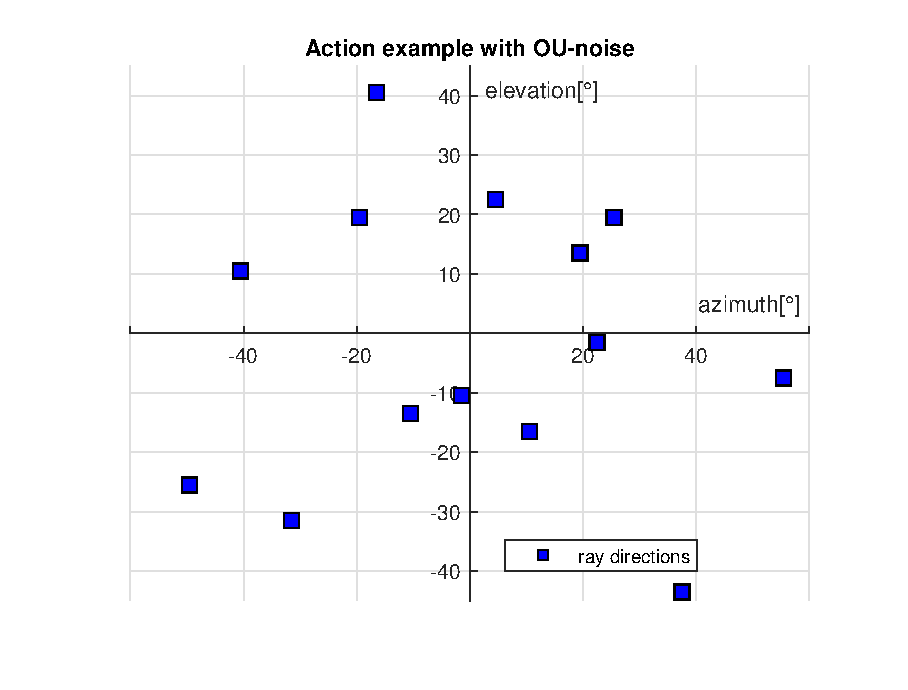
\includegraphics[width=\linewidth]{fig/right_action.eps}
\end{subfigure}
\captionsetup{width=1\textwidth}
\caption[Difference between exploration methods]{Difference between actions made by agents with different exploration methods. Left figure is an example of action made by an agent with Gaussian noise used for exploration. The action in the right figure is taken by agent trained using Ornstein-Uhlenbeck noise.}
\label{fig:expdiff}
\end{figure}

\subsection{Stochastic planning agent}
There is an obvious issue with the deterministic actor. For efficient exploring of ground truth map is required to hit as many unique voxels as possible. Thus making several similar actions in a row is not a good strategy. Unfortunately, except first few timestamps of every drive, there is not a big difference between two subsequent observations. It is hard for a neural network to make two different outputs for two similar inputs. The solution to this problem could be a stochastic agent. Stochastic agent outputs parameters of beta distribution and preserves actor-critic framework. The architecture of stochastic agent is similar to DDPG from the previous subsection, only difference is that agent now outputs only two values - distribution parameters. Action is then sampled with distribution probabilities.

\clearpage
\subsection{Comparison of methods}
